% !TEX TS-program = pdflatex
% !TEX encoding = UTF-8 Unicode

% This is a simple template for a LaTeX document using the "article" class.
% See "book", "report", "letter" for other types of document.

\documentclass[11pt]{article} % use larger type; default would be 10pt

\usepackage[utf8]{inputenc} % set input encoding (not needed with XeLaTeX)

%%% Examples of Article customizations
% These packages are optional, depending whether you want the features they provide.
% See the LaTeX Companion or other references for full information.

%%% PAGE DIMENSIONS
\usepackage{geometry} % to change the page dimensions
\geometry{a4paper} % or letterpaper (US) or a5paper or....
% \geometry{margin=2in} % for example, change the margins to 2 inches all round
% \geometry{landscape} % set up the page for landscape
%   read geometry.pdf for detailed page layout information

\usepackage{graphicx} % support the \includegraphics command and options

% \usepackage[parfill]{parskip} % Activate to begin paragraphs with an empty line rather than an indent

%%% PACKAGES
\usepackage{booktabs} % for much better looking tables
\usepackage{array} % for better arrays (eg matrices) in maths
\usepackage{paralist} % very flexible & customisable lists (eg. enumerate/itemize, etc.)
\usepackage{verbatim} % adds environment for commenting out blocks of text & for better verbatim
\usepackage{subfig} % make it possible to include more than one captioned figure/table in a single float
% These packages are all incorporated in the memoir class to one degree or another...

%%% HEADERS & FOOTERS
\usepackage{fancyhdr} % This should be set AFTER setting up the page geometry
\pagestyle{fancy} % options: empty , plain , fancy
\renewcommand{\headrulewidth}{0pt} % customise the layout...
\lhead{}\chead{}\rhead{}
\lfoot{}\cfoot{\thepage}\rfoot{}

%%% SECTION TITLE APPEARANCE
\usepackage{sectsty}
\allsectionsfont{\sffamily\mdseries\upshape} % (See the fntguide.pdf for font help)
% (This matches ConTeXt defaults)

%%% ToC (table of contents) APPEARANCE
\usepackage[nottoc,notlof,notlot]{tocbibind} % Put the bibliography in the ToC
\usepackage[titles,subfigure]{tocloft} % Alter the style of the Table of Contents
\usepackage{framed}
\renewcommand{\cftsecfont}{\rmfamily\mdseries\upshape}
\renewcommand{\cftsecpagefont}{\rmfamily\mdseries\upshape} % No bold!

%%% END Article customizations

%%% The "real" document content comes below...

\title{The Monty Hall Problem}
\author{Dublin R}


\begin{document}
\maketitle

\section{The Monty Hall Problem}
\begin{figure}[h!]
\centering

\includegraphics[width=0.5\linewidth]{./MH1}
\caption{}
\label{Monty Hall}
\end{figure}

Suppose that there are three closed doors on the set of the \textbf{\textit{Let's Make a Deal}}, a TV game
show presented by Monty Hall. Behind one of these doors is a car; behind the other two are
goats. The contestant does not know where the car is, but Monty Hall does.

The contestant selects a door, but not the outcome is not immediately evident. Monty
opens one of the remaining "wrong" doors. If the contestant has already chosen the correct
door, Monty is equally likely to open either of the two remaining doors.

After Monty has shown a goat behind the door that he opens, the contestant is always given the option to switch doors. 

\begin{figure}
\centering
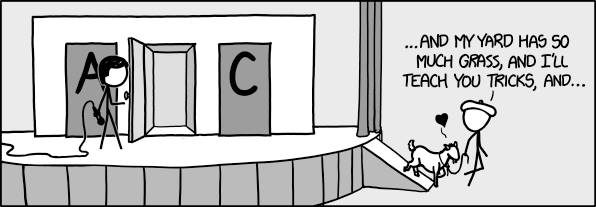
\includegraphics[width=0.7\linewidth]{./MontyHall}
\caption{}
\label{fig:MH1}
\end{figure}


\item What is the probability of winning the car if she stays with her original choice? 
\item What if she decides to switch?
\end{itemize}

\subsection{Marilyn Vos Savant}
The Monty Hall problem 

Perhaps the best-known event involving vos Savant began with a question in her 9 September 1990 column:


Suppose you're on a game show, and you're given the choice of three doors. Behind one door is a car, behind the others, goats. You pick a door, say 1, and the host, who knows what's behind the doors, opens another door, say 3, which has a goat. He says to you, "Do you want to pick door 2?" Is it to your advantage to switch your choice of doors?

—Craig F. Whitaker Columbia, Maryland, 

This question is referred to as "the Monty Hall problem" because of its similarity to scenarios on the game show Let's Make a Deal, and its answer existed long before being posed to vos Savant, but was used in her column. Vos Savant answered arguing that the selection should be switched to door 2 because it has a 2 in 3 chance of success, while door 1 has just 1 in 3. Or to summarise, 2 in3 of the time the opened door 3 will indicate the location of the door with the car (the door you hadn't picked and the one not opened by the host). 

Only 1 in3 of the time will the opened door 3 mislead you into changing from the winning door to a losing door. These probabilities assume you change your choice each time door 3 is opened, and that the host always opens a door with a goat. This response provoked letters of thousands of readers, nearly all arguing doors 1 and 2 each have an equal chance of success. A follow-up column reaffirming her position served only to intensify the debate and soon became a feature article on the front page of The New York Times. Parade received approximately 10,000 letters from readers who believed that vos Savant was wrong – among the ranks of dissenting arguments \textbf{\textit{were nearly 1,000 letters carrying signatures with PhDs}}.

Under the "standard" version of the problem, the host always opens a losing door and offers a switch. In the standard version, vos Savant's answer is correct. However, the statement of the problem as posed in her column is ambiguous. The answer depends upon what strategy the host is following. For example, if the host operates under a strategy of only offering a switch if the initial guess is correct, it would clearly be disadvantageous to accept the offer. If the host merely selects a door at random, the question is likewise very different from the standard version. Vos Savant addressed these issues by writing the following in Parade Magazine, "the original answer defines certain conditions, the most significant of which is that the host always opens a losing door on purpose. Anything else is a different question."

In vos Savant's second followup, she went further into an explanation of her assumptions and reasoning, and called on school teachers to present the problem to each of their classrooms. In her final column on the problem, she announced the results of more than a thousand school experiments. Nearly 100\% of the results concluded that it pays to switch. Of the readers who wrote computer simulations of the problem, 97\% reached the same conclusion. A majority of respondents now agree with her original solution, with half of the published letters declaring the letter writers had changed their minds.

\subsection{The Sample Space}
One way to think about this problem is to consider the sample space, which Monty alters by opening one of the doors that has a goat behind it. In doing so, he effectively removes one of the two losing doors from the sample space.
We will assume that there is a winning door and that the two remaining doors, A and B, both have goats behind them. There are three options:


\item The contestant first chooses the door with the car behind it. She is then shown either door A or door B, which reveals a goat. If she changes her choice of doors, she loses. If she stays with her original choice, she wins.

\item The contestant first chooses door A. She is then shown door B, which has a goat behind it. If she switches to the remaining door, she wins the car. Otherwise, she loses.
\item The contestant first chooses door B. She is then is shown door A, which has a goat behind it. If she switches to the remaining door, she wins the car. Otherwise, she loses.
\end{itemize}
Each of the above three options has a 1/3 probability of occurring, because the contestant is equally likely to begin by choosing any one of the three doors. In two of the above options, the contestant wins the car if she switches doors; in only one of the options does she win if she does not switch doors. When she switches, she wins the car twice (the number of favorable outcomes) out of three possible options (the sample space). Thus the probability of winning the car is 2/3 if she switches doors, which means that she should always switch doors - unless she wants to become a goatherd.
\subsection{Counter Intuitive Result}
This result of 2/3 may seem counterintuitive to many of us because we may believe that the probability of winning the car should be 1/2 once Monty has shown that the car is not behind door A or door B. Many people reason that since there are two doors left, one of which must conceal the car, the probability of winning must be 1/2. This would mean that switching doors would not make a difference. As we've shown above through the three different options, however, this is not the case.


%------------------------------------------------%
\subsection{ \texttt{R} Implementation (part 1)}
We have 3 doors to choose from, so we will dene a numeric sequence between 1 and 3. The
command \texttt{sample(,n)} takes a sample of size n from a specified set of values. Here we just
want to select one door to be our \textbf{\textit{correct door}} and another to be \textbf{\textit{selected}} door (i.e. the door that the contestant selects).

These events are independent. For the sake of simplicity, we will perform the selection for both doors separately, but this can be implemented in one command.

\begin{verbatim}}
Doors = 1:3 
Correct = sample(Doors,1)
Choice = sample(Doors,1)
\end{verbatim}



\begin{verbatim}
> Doors
[1] 1 2 3
> Correct
[1] 1
> Choice
[1] 3
\end{verbatim}

%--------------------------------------------%

\subsection{ \texttt{R} Implementation (part 2)}
In this part, we will use the set theory commands \texttt{union()} and \texttt{setdiff()}. Another related command is \texttt{intersect()}, but we will not be using it here.

These commands are very simple, and can be best demonstrated with a simple example.

\begin{verbatim}
X <- 1:6
Y <- 5:9
union(X,Y)
intersect(X,Y)
setdiff(X,Y)
setdiff(Y,X)
\end{verbatim}

The output from these commands looks like this:
\begin{verbatim}
> X
[1] 1 2 3 4 5 6
> Y
[1] 5 6 7 8 9
>
> union(X,Y)
[1] 1 2 3 4 5 6 7 8 9
> intersect(X,Y)
[1] 5 6
> setdiff(X,Y)
[1] 1 2 3 4
> setdiff(Y,X)
[1] 7 8 9
\end{verbatim}
Going back to the Monty Hall problem. The Set Theory commands aver very useful in that they can avoid a lot of programming control statements to account for various scenarios. A wrong door must be selected to be opened. The door selected by the contestant can't be
chosen. First let us select the doors that must stay closed, then find the doors that the contestant can choose from.

\begin{verbatim}
StayClosed = union(Correct, Choice)
CanOpen = setdiff(Doors, StayClosed)
\end{verbatim}

%-------------------------------------------------------%

\subsection{Using the \texttt{sample command}}


The \texttt{R} command \texttt{sample()} poses an interesting problem. Lets look at the help file to see what it is.
Create a single element vector (let's call it \textbf{Vec}, with that single element being 4. 

Now sample a single value from that data set. You may expect to get 4 each time, as it is the only element in the set but \texttt{R} doesnt work that way in this instance.

\begin{verbatim}
Vec=c(4)
sample(Vec,1)
\end{verbatim}

Instead \texttt{R} interprets the argument 4 as the upper bound of a sequence of four integers (i.e. the sample space is 1 to 4)
\begin{verbatim}
> sample(Vec,1)
[1] 3
> sample(Vec,1)
[1] 4
> sample(Vec,1)
[1] 1
\end{verbatim}

Problems will arise when the number of elements in the \textbf{CanOpen} set of numbers is one.
When there are more than one, things will work fine.
%-------------------------------------------------------------------------------------%
To overcome thisproblem, we need some control statements.

\item  If there are two elements in the data set, we just select one of them at randomm using the \texttt{sample()} command.
\item If there is only one element in the data set we avoid using the \texttt{sample()} command, and instead use the assignment operator.
\end{itemize}
We wish to select a door for opening, to reveal the goat.

\begin{verbatim}
if(length(CanOpen)>1)
{
Open = sample(CanOpen,1)
}else {Open=CanOpen}
Open # This door reveals a goat
\end{verbatim}

%-------------------------------------------------------------------------------------%
\subsection{Stick or Switch?}
There are two unopened doors. One is the correct door, but which one? Should the contestant \textbf{stick} or \textbf{switch} ?


\begin{verbatim}
NotOpen = setdiff(Doors,Open)

Stick = Choice
# Stick with the original choice

Switch = setdiff(NotOpen,Choice)
# Switch to the other door
\end{verbatim}


Was sticking the right decision? Or was switching?


\begin{verbatim}
# Was sticking the right decision? Or was switching?
# The following logicial statements will tell us.
Stick==Correct
Switch==Correct
\end{verbatim}


An answer of 1 means that decision would have been correct. Equivalently, a response of 0 indicates a bad decision.
%-------------------------------------------------------------------%


\subsection{ Writing a Function}
We are going to create a function \texttt{MHfunc()} to help us simulate a solution for the Monty Hall Problem. The function is constructed using R code we have seen already. The output of the
function is returned as a data frame, with 7 columns:


\item Correct : The number of the correct door.
\item Choice : The door that the contestant chose originally, and the door selected if the contestant decided to "stick".
\item Open : The door Monty Hall opens to reveal a goat
\item StickDoor : The door that the contestant chose originally, and the door selected if the contestant decided to "stick".
\item SwitchDoor : The door selected if the contestant chose to "switch".
\item Stick: Was Sticking a good decision (1 for yes, 0 for no)
\item Switch : Was Switching a good decision (1 for yes, 0 for no)
\end{itemize}
The output looks like this:
\begin{verbatim}
> MHfunc()
   Correct     Choice Open(goat)  StickDoor SwitchDoor      Stick     Switch 
         2          2          1          2          3          1          0 
> MHfunc()
   Correct     Choice Open(goat)  StickDoor SwitchDoor      Stick     Switch 
         1          2          3          2          1          0          1 
> MHfunc()
   Correct     Choice Open(goat)  StickDoor SwitchDoor      Stick     Switch 
         1          2          3          2          1          0          1
\end{verbatim}



\begin{verbatim}
MHfunc <- function(numdoors=3){
Doors = 1:numdoors
Correct = sample(Doors,1)
Choice = sample(Doors,1)
StayClosed = union(Correct, Choice)
CanOpen = setdiff(Doors, StayClosed)

#Open the Door with a Goat
if(length(CanOpen)>1)
{
Open = sample(CanOpen,1) #Problem here
}else {Open=CanOpen}

NotOpen = setdiff(Doors,Open)

#Stick or Switch
Stick = Choice
Switch = setdiff(NotOpen,Choice)
Stick.Decision= as.numeric(Stick==Correct)
Switch.Decision = as.numeric(Switch==Correct)

#Preparing the Output
MHoutput=c(Correct,Choice,Open,Stick,Switch,
 Stick.Decision,Switch.Decision)

names(MHoutput)= c("Correct","Choice","Open(goat)","StickDoor",
 "SwitchDoor","Stick","Switch")
return(MHoutput)
}
\end{verbatim}


%---------------------------------------------------------------%

\subsection{ A Simulation Study of the Monty Hall Problem}
Let us perform a simulation study of the Monty Hall problem. We are putting the code we have
written already, placed in a for loop, although we alter the ending to make for more readable
output.

\begin{verbatim}
#Initialise Counters
StickCount = 0   
SwitchCount = 0

#How many Trials?
M=1000

# a For loop
for(i in 1:M)
	{
	output=MHfunc()

	StickCount = StickCount + output[6]
	SwitchCount = SwitchCount + output[7]
	}
StickCount
SwitchCount
\end{verbatim}


The output of this program would look like this. The proportion is approximately 2 to 1 in
favour of the switching option.
\begin{verbatim}
> StickCount
[1] 323
> SwitchCount
[1] 677
\end{verbatim}


\end{document}
